\documentclass[logo,civil,propuesta]{tesis-pregrado}
% opciones: logo,dosguias,civil,ejecucion,propuesta,txfonts

\keywords{XML; Key Implication}

\begin{document}
\baselineskip 23pt
% ----------------------------------------------------------
% ----------- PARTE INICIAL --------------------------------
\thispagestyle{empty}
% Rellenar con la informacion personal y del trabajo

\titulo{Desarrollo de aplicaci\'on para procesos de producci\'on y mantenimiento de impresoras 3D FDM utilizando Octoprint}

\autor{Pablo Alejandro Ruz Donoso }
\email{pablo.ruz@usach.cl}
\telefono{+569 72369058}
\run{17,874.835-1}
\annoingreso{2018}

\fecha{Jueves}{16}{julio}{2020}

\profesorguia{Pablo Alvarado M.}


\ciudad{Santiago}
\pais{Chile}

\makecubierta

\makecopyright % si es propuesta no se mostrará
% ----------------------------------------------------------
% ----------- PRIMERA PARTE --------------------------------
\frontmatter
% ### Resumen e Indices ####

\begin{gracias}

\end{gracias}
\dedicatoria{
Dedicado a...
}

\resumenCastellano{
Contrariamente a la creencia popular, Lorem Ipsum no es simplemente texto aleatorio. Tiene sus raíces en una pieza de la literatura clásica latina de 45 aC, por lo que es más de 2000 años de antigüedad. Richard McClintock, un profesor de latín en Hampden-Sydney College en Virginia, encontró una de las palabras latinas más oscuros, Consectetur, a partir de un pasaje de Lorem Ipsum, y pasando por la cita de la palabra en la literatura clásica, descubrió la fuente indudable. Lorem Ipsum viene de las secciones 1.10.32 y 1.10.33 de "De finibus" (Los Extremos del Bien y del Mal) por Cicero, escrito en el año 45 aC. Este libro es un tratado sobre la teoría de la ética, muy popular durante el Renacimiento. La primera línea de Lorem Ipsum, "Lorem ipsum dolor sit amet ..", viene de una línea en la sección 1.10.32.

La porción estándar de Lorem Ipsum usado desde el año 1500. A continuación se reproduce para los interesados. Las secciones 1.10.32 y 1.10.33 de "De finibus" por Cicerón también se reproducen en su forma original exacta, acompañadas por versiones en Inglés de la traducción en 1914 por H. Rackham.

\vspace*{0.5cm}
\KeywordsES{Palabras; Claves}
}

\newpage

\resumenIngles{
Contrary to popular belief, Lorem Ipsum is not simply random text. It has roots in a piece of classical Latin literature from 45 BC, making it over 2000 years old. Richard McClintock, a Latin professor at Hampden-Sydney College in Virginia, looked up one of the more obscure Latin words, consectetur, from a Lorem Ipsum passage, and going through the cites of the word in classical literature, discovered the undoubtable source. Lorem Ipsum comes from sections 1.10.32 and 1.10.33 of "de Finibus Bonorum et Malorum" (The Extremes of Good and Evil) by Cicero, written in 45 BC. This book is a treatise on the theory of ethics, very popular during the Renaissance. The first line of Lorem Ipsum, "Lorem ipsum dolor sit amet..", comes from a line in section 1.10.32.

The standard chunk of Lorem Ipsum used since the 1500s is reproduced below for those interested. Sections 1.10.32 and 1.10.33 from "de Finibus Bonorum et Malorum" by Cicero are also reproduced in their exact original form, accompanied by English versions from the 1914 translation by H. Rackham.

\vspace*{0.5cm}
\KeywordsEN{Key; words}
}

\pagestyle{fancy}
\fancyhead[L]{\slshape \leftmark}
\fancyhead[C]{}
\fancyhead[R]{\thepage}
\tableofcontents        %% Indice general
\listoffigures          %% Indice de figuras
\listoftables           %% Indice de tablas
\listofalgorithms       %% Indice de algoritmos
% ----------- SEGUNDA PARTE --------------------------------
\mainmatter
% ### Configuración del header ###
\pagestyle{fancy}
\fancyhead[L]{\slshape \leftmark}
\fancyhead[C]{}
\fancyhead[R]{\thepage}
\pagenumbering{arabic}
% ### Capitulos de la tesis ###
\chapter{Introducci\'on}
\label{cap:intro}

\section{Antecedentes y motivaci\'on}
\label{intro:motivacion}

 \ldots 


\section{Descripci\'on del problema}
\label{intro:problema}



\section{Soluci\'on propuesta}
\label{intro:solucion}


\section{Objetivos y alcance del proyecto}
\label{intro:objetivos}

\subsection{Objetivo general}

Diseñar una aplicación de gestión de la producción y el mantenimiento correctivo y preventivo para la optimización de procesos de impresión 3D FDM.

\subsection{Objetivos espec\'ificos}

Para la consecución del objetivo general, se plantean las siguientes metas intermedias:

\begin{enumerate}
 
	\item Determinar las variables implicadas en el proceso que permiten obtener indicadores.
	\item Investigar compatibilidad entre hardware, software, protocolos de comunicación, y códigos de programación a utilizar.
	\item Elaborar registros y fichas técnicas de impresoras 3D.
	\item Establecer relaciones matemáticas que permitan entregar indicadores relevantes para la producción y mantenimiento.
	\item Diseñar funciones que permitan gestionar los datos de hardware y software para determinación de indicadores.
	\item Diseñar interfaz de aplicación orientado al usuario. 
	
\end{enumerate} \ldots 
\subsection{Alcances}

Se pretende desarrollar una Interfaz Programable de Aplicación utilizando como base el software Octoprint, pudiendo controlar, monitorizar en tiempo real el funcionamiento de varias impresoras 3D, y entregar indicadores para gestionar la producción y el mantenimiento de las máquinas. Para esto, se toman en cuenta los siguientes alcances:

\begin{enumerate}
	\item Emplear metodologías ágiles para el diseño.
	\item Utilizar softwares y herramientas de código abierto.
	\item Trabajar en una plataforma cliente/servidor.
	\item Diseñar un sistema enfocado en el usuario.
	\item Tomar las entradas de impresoras, lista de piezas, tiempos de producción, peso de filamento y tiempo de actividad. 
	\item Configurar planificación y frecuencia de mantenimientos autónomos y preventivos.
	\item Configurar planificación y emitir órdenes de producción.
	\item Emitir reportes y consultas sobre el estado de las órdenes de producción y mantenimiento. 


\end{enumerate}  

\section{Metodolog\'ia y herramientas utilizadas}
\label{intro:metodologia}

\subsection{Metodolog\'ia}


\subsection{Herramientas de desarrollo}


\section{Resultados Obtenidos}
\label{intro:resultados}


\section{Organizaci\'on del documento}
\label{intro:organizacion}



%--------Preliminares
%--------Emir Muñoz Jiménez
%--------13-10-2010

\chapter{Marco Te\'orico}
\label{cap:preliminares}

\section{Impresión 3D}

 A diferencia de las técnicas principales que se emplean desde hace algunos años en la fabricación de objetos, que se encargan de sustraer, combinar, o deformar paulatina y controladamente materia hasta llegar a una pieza final, la impresión 3D funciona de un modo completamente distinto. La pieza se crea en un solo paso, capa por capa, a un ritmo medio de uno a dos centímetro de altura por hora; el objeto creado puede constar de mecanismos internos (como rodamientos de bolas), formas tejidas y entrelazadas, o incluso huecos y curvas \citep{Berchon2014}. Pues bien, todas las impresoras 3D, están basadas sobre el mismo principio: un modelo digital es transformado a un objeto físico de 3 dimensiones por adición de material en capas. Esto se conoce alternativamente como \textit{Manufactura Aditiva} \citep{tresdhub2018}. Este tipo de fabricación también se puede englobar dentro de lo que se denomina \textit{Fabricación digital}, cuyo principio básico es la transformación de la información  desde el mundo físico al digital. Según \citep{jorquera2016}, la fabricación digital incluye los siguientes sistemas y tecnologías:\\
 
 \begin{enumerate}
 	
	\item Sistemas integrados: Es un \textit{hardware} electrónico diseñado específicamente para llevar a cabo una o pocas tareas definidas. Las impresoras llevan un sistema electrónico integrado que utilizan para controlar los motores paso a paso que alimentan el papel, recibir información de los sensores de temperatura y finales de carrera, o que mandan al cabezal de impresión.
	\item Sistemas CNC (\textit{Computer Numeric Control} - control numérico computarizado): Es el control numérico de un sistema de automatización que se utiliza para controlar diferentes máquinas herramienta. Este sistema ha revolucionado la industria gracias a la simplificación del \textit{software} de diseño en conjunto con los lenguajes de programación como el \textit{.gcode}. Esencialmente, un sistema CNC es cualquier sistema que utiliza un ordenador para controlar los movimientos de una máquina.
	\item Software CAD (\textit{Computer Aided Design}- diseño asistido por computador): es, en esencia, un programa que sirve para la creación, edición análisis y visualización de modelos tridimensionales.  
	\item Internet: Los programas CAD actuales disponen de herramientas de trabajo colaborativo en red, de esta manera se define el producto y el proceso de fabricación de forma simultánea.\\

  \end{enumerate}

En la misma línea, y dependiendo de la profundidad técnica que el proceso de fabricación necesite, se agregan los sistemas \citep{leao2017}:

\begin{enumerate}
	\item Software CAE (\textit{Computer Aided Engineering} - Ingeniería Asistida por computador): Son los programas mayoritariamente usados para las tareas de análisis de ingeniería. Estos \textit{softwares}, a través de métodos numéricos como el método de elementos finitos o dinámica de fluidos computacional, se utilizan para, por ejemplo, analizar la robustez y el funcionamiento de ensambles de piezas.
	\item Software CAM (\textit{Computer Aided Manufacturing}- Manufactura Asistida por computador): Corresponde a programas que controlan las herramientas de máquinas de control numérico relacionadas con el proceso de manufactura a realizar, generando un código específico para el producto a fabricar. 

\end{enumerate}

%Figura: Expectativas impresi\'on 3D 
\begin{figure}[tp]
  \centering
    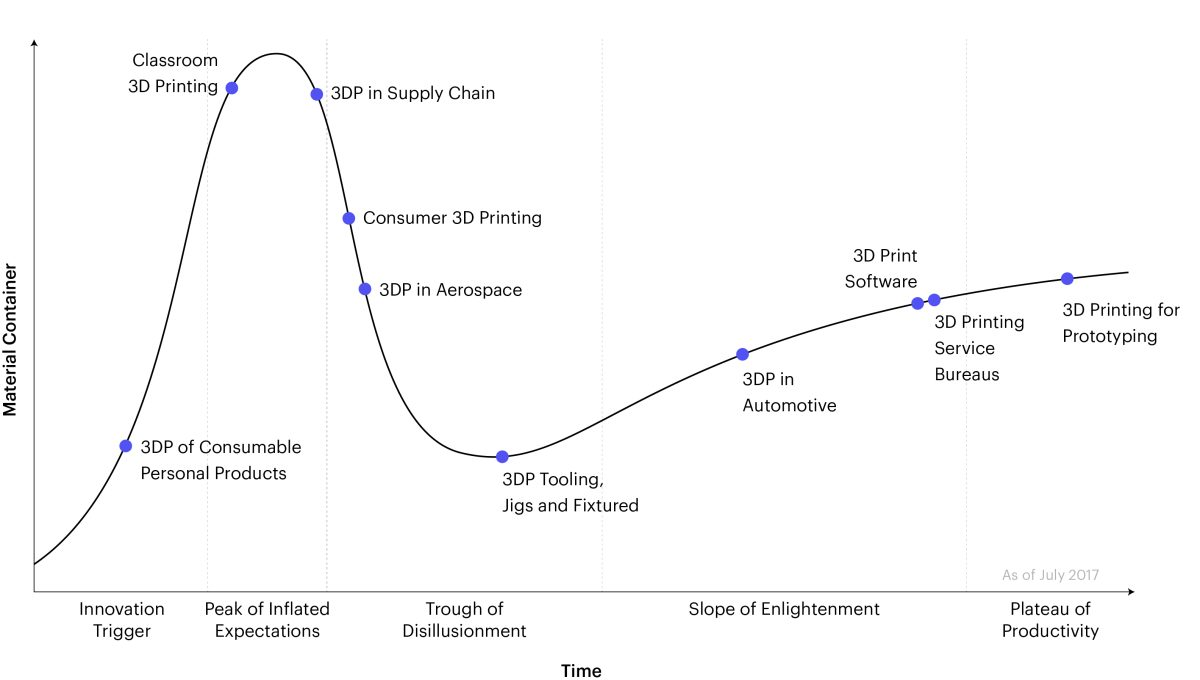
\includegraphics[width=\textwidth]{images/The3Dprintinghypecycle.png}
  \caption{Mi Figura}
  \label{fig:ejemplo}
\end{figure}

% Figura: \'Arbol XML 1
%\begin{figure}[tp]
%  \centering
%  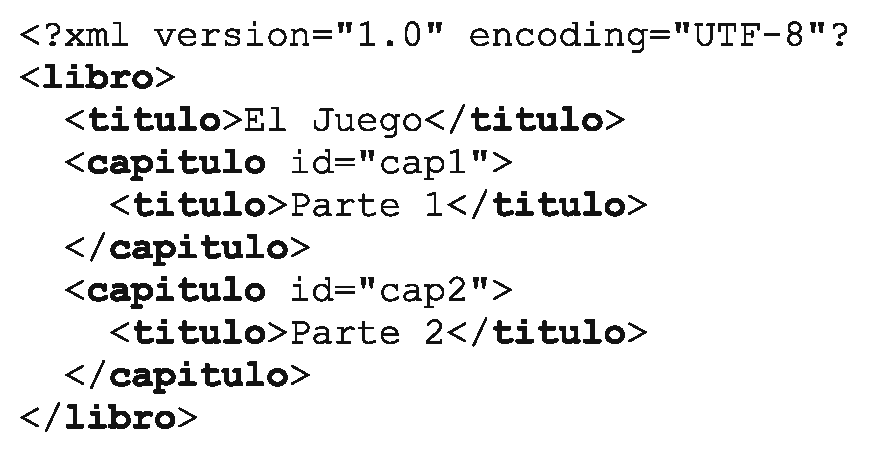
\includegraphics[scale=.5]{images/XML-document-example1}
%  \caption{\em Modelo de árbol para un documento XML.}
%  \label{fig:xml-tree-exa1}
%\end{figure}


\subsection{Historia de la impresión 3D}

El comienzo de la generación del concepto de impresión 3D puede ser rastreado al año 1976, a partir de la creación de la primera impresora a tinta por inyección \citep{maxey2013}. La utilización de la inyección de tinta abrió la pregunta respecto a qué tipo de materiales podían ser utilizados con esta tecnología, y cómo los mecanismos presentes en la época podían ser adaptados para abrir la posibilidad de ocupar otras materias primas. En Mayo de 1981, el Dr. Hideo Kodama del Instituto de Investigación Industrial del Municipio de Nagoya publicó detalles relativos a la técnica de prototipado rápido. Esta investigación se considera como la primera publicación que describe la técnica de fabricación capa a capa propia de los procesos de impresión 3D; no obstante, los desarrollos de Kodama no llegaron a ser materializados debido a problemas encontrados en el proceso de fundido de material. \citep{tresdsourced2020}. Paralelamente, la idea de ``máquinas de prototipado rápido'' continuó su desarrollo en Francia, por Jean-Claude André, Oliver de Witte y Alain le Méhauté. En la primera mitad de la década de los 80, le Méhauté investigaba en la empresa Alcatel sobre partes y piezas generadas a partir de la geometría fractal, y la manera en que éstas podrían ser fabricadas dada su complejidad de forma.
De Witte, quien era también investigador de Alcatel en el área de luz láser, propuso a le Méhauté que algunos líquidos compuestos por ciertos monómeros podían ser curados y transformados en sólidos tras la aplicación de luz láser, convirtiéndose en el primer paso para la construcción efectiva de máquinas de prototipado rápido a través de el proceso de Estereolitografía. Ambos compartieron el resultado de sus avances con André, que en ese tiempo trabajaba en el Centro Nacional Frances de Investigación Científica, para ya el año 1984 inscribir la patente de su desarrollo. Infortunadamente, el grupo debe abandonar el proyecto debido a problemas con la solidificación del material y poca rentabilidad desde la perspectiva económica \citep{alltresdp2018}.\

Con solo tres semanas de diferencia respecto a los investigadores franceses, Charles `Chuck' Hull solicita la patente del proceso de Esterolitografía con nuevos avances, como la utilización del formato STL (Standard Triangle Language) y la laminación digital de objetos. A diferencia del a Esterolitografía francesa, el método de Hull utiliza luz ultravioleta para el curado de fotopolímeros. El año 1986, obtenida su patente, Hull forma la empresa \textit{3D Systems} y lanza la primera impresora 3D, la \textit{SLA-1}, el año 1987 \citep{tresdsourced2020}.


\subsection{Métodos de impresión 3D}

\subsection{Impresoras 3D FDM}

\subsection{Tipologías de impresión 3D FDM}

\section{Mantenimiento}

\section{Confiabilidad}

La confiabilidad puede ser definida como la "confianza que se tiene de que un componente, equipo o sistema desempeñe su función básica, durante un periodo de tiempo preestablecido, bajo condiciones estándares de operación; otra definición es la probabilidad de que un ítem pueda desempeñar su función requerida durante un intervalo establecido y bajo condiciones de uso definidas \citep{dairo2016}. Esta segunda definición da a entender que existen herramientas estadísticas que pueden ser utilizadas para obtener información acerca del cómo se comportan las fallas en el tiempo.

\subsection{Función densidad de probabilidad}

La función densidad de probabilidad puede describir la distribución de la probabilidad de una variable aleatoria continua $X$. Así, una función de densidad de probabilidad es una función tal que:

\begin{enumerate}
\item $f(x)\geqslant 0$
\item $\int_{-\infty}^{\infty}f(x)dx=1$
\item $P(a\geqslant X \geqslant b)=\int_{a}^{b}f(x)dx=$ área bajo $f(x$) de $a$ a $b$, para cualquier $a$ y $b$.
\end{enumerate}

Esta función proporciona una descripción simple de las probabilidades asociadas a una variable aleatoria.
\subsection{Media y varianza de una variable continua}

Si se tiene que $X$ es una variable aleatoria continua con función de densidad de probabilidad $f(x)$, se define la Media de $X$ como:

\begin{equation*}
\mu=E(X)=\int_{-\infty}^{\infty}xf(x)dx
\end{equation*}

Asimismo, la Varianza de $X$:

\begin{equation*}
\sigma^2=V(X)=\int_{-\infty}^{\infty}(x-\mu)^{2}f(x)dx=\int_{-\infty}^{\infty}x^{2}f(x)dx-\mu^2
\end{equation*}

La Desviación Estandar:

\begin{equation*}
\sigma=\sqrt{V(X)}
\end{equation*}

\subsection{Distribución normal}

Variables aleatorias con medias y varianzas diferentes pueden modelares por medio de funciones de densidad de probabilidad normal, con la elección adecuada del centro y anchura de la curva. La función de densidad de probabilidad normal se define como:

\begin{equation*}
f(x)=\frac{1}{\sqrt{2\pi\sigma}}e^{\frac{-(x-\mu)^2}{2\sigma^2}}  ,  -\infty<x<\infty
\end{equation*}

tiene una distribución normal con parámetros $\mu$, donde $-\infty<\mu<\infty$, y $\sigma>0$.\\

Además,
\begin{equation*}
E(X)=\mu , V(x)=\sigma^2
\end{equation*}

\subsection{Distribución exponencial}

La distribución exponencial debe su nombre a la función exponencial de la función de densidad de probabilidad. Así, la variable aleatoria $X$ (que es igual a la distancia entre conteos sucesivos de un proceso de Poisson con media $\lambda>0$ tiene una distribución exponencial con parámetro $\lambda$:

\begin{equation*}
f(x)=\lambda e^{-\lambda x}, 0<x<\infty
\end{equation*}

Si la variable tiene una distribución exponencial con parámetro $\lambda$:

\begin{equation*}
E(x)=\frac{1}{\lambda}, V(X)=\frac{1}{\lambda^2}
\end{equation*}

\subsection{Distribución de Weibull}

La distribución de Weibull se utiliza con frecuencia para modelar el tiempo hasta que ocurre una falla en algún sistema. La variable aleatoria $X$ con función de densidad de probabilidad:

\begin{equation*}
f(x)=\frac{\beta}{\delta}\left( \frac{x}{\delta} \right)^{\beta-1}e^{\left( \frac{x}{\delta} \right)}{}^\beta
\end{equation*}

tiene una distribución de Weibull con parámetro de escala $\delta>0$ y parámetro de forma $\beta>0$.



\subsection{Historia y evolución del mantenimiento}

\subsection{Tipos de mantenimiento}

\subsection{GMAO}

\section{Lean Manufacturing}

\subsection{Historia Lean Manufacturing}

\subsection{Herramientas de mantenimiento}

\section{Design Thinking y Scrum}

\subsection{Metodologías ágiles}

\subsection{Scrum}

\subsection{Design Thinking}

\subsection{Fases del Design Thinking}

\subsection{Herramientas para diseño de Software}

\section{Desarrollo de Software}

\subsection{Programación orientada a objetos}

\subsection{Lenguajes de programación}

\subsection{Arquitectura Cliente-Servidor}

\subsection{API}

\subsection{Ordenadores de placa reducida}

 \ldots 

 

% Figura: \'Arbol XML 1
%\begin{figure}[tp]
%  \centering
%  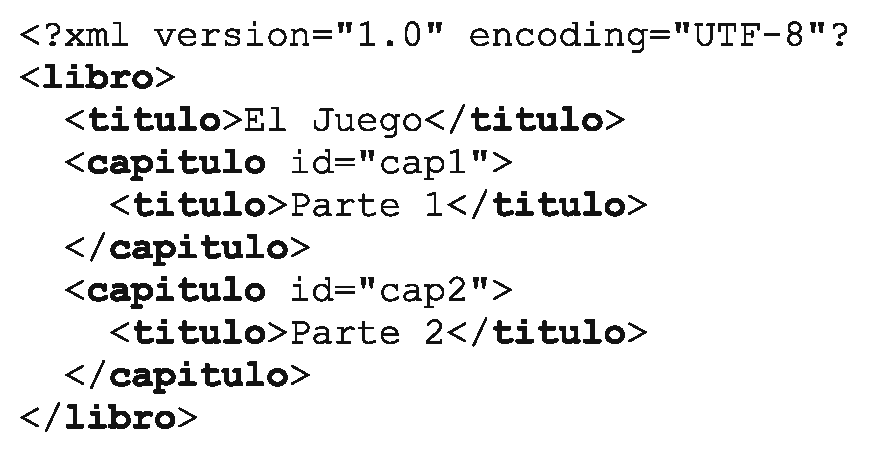
\includegraphics[scale=.5]{images/XML-document-example1}
%  \caption{\em Modelo de árbol para un documento XML.}
%  \label{fig:xml-tree-exa1}
%\end{figure}






% ----------- TERCERA PARTE --------------------------------
\backmatter %Elimina la numeración
% ### Bibliografía de este documento ###
\bibliographystyle{apalike}
\bibliography{bibliografia}
% ----------------------------------------------------------
% ----------- CUARTA PARTE ---------------------------------
\appendix
\addappheadtotoc %agregar Apéndice al índice. Si no tiene apéndices COMENTAR o BORRAR
% \noappendicestocpagenum %quitar número de páginas a los apéndices
% ### ANEXOS ###
\chapter{Título del apéndice ejemplo}
\label{finales:apendice1}
El 15 de junio del 2012 la Agencia Acreditadora Colegio de Ingenieros de Chile S.A., otorga la acreditación de la carrera de Ingeniería Civil Informática de la Universidad de Santiago de Chile sede Santiago, en sus jornadas diurna y vespertinas por un plazo de 5 años. % Manuales de Usuario
\end{document}
%\\end
